\documentclass[english]{article}

\usepackage{babel}
\usepackage{graphicx}
\usepackage{times}
\usepackage{pifont}
\usepackage[margin=1in]{geometry}
\usepackage{eurosym}
\usepackage{fancyhdr}
\usepackage[hidelinks]{hyperref}

\pagestyle{fancy}
\fancyhf{}


%HEADER
%**************************************************************************************
\pagestyle{fancy}
\fancyhf{}
%**************************************************************************************
\lhead{GSM base station measurements}		 	 
\rhead{Laboratory Work in Telecommunications} 
\lfoot{EFA12SF}
\cfoot{\thepage}
\rfoot{Dmitry Boronin\\ Nikolay Arsenov\\ Alexey Tukalo}
%**************************************************************************************

\date{}
\setlength\parindent{0pt}

\begin{document}

\title{\vspace{2in}GSM base station measurements\\
\small for Laboratory Work in Telecommunications\\
\vspace{0.5in}
\includegraphics{savonia.jpg}}

\nopagebreak
\maketitle


\vspace{3in}

\author{
\begin{flushright}
Dmitry Boronin, Nikolay Arsenov, Alexey Tukalo,\\
EFA12SF,\\
Information Technology,\\
Savonia University of Applied Sciences
\end{flushright}
}

\date{\today}
\thispagestyle{empty}

\newpage
\setcounter{page}{1}
\setcounter{tocdepth}{2}
\tableofcontents

\newpage

%MAIN CONTENT ******************************************************************************************************************
\section{General information about MMI}
The user via the BTS Nokia Man-Machine Interface can control the Base Transceiver Station (BTS) equipment. (fig. 1) Controlling can be done locally at the BTS site and also remotely from the Base Station Controller (BSC) or Network Management System (NMS/2000). The Talk-family and Nokia Prime Site BTS Man-Machine Interface software includes three applications: the MMI version 6.0.1, the MMIDATA version 6.0.1 and the HWINFO version 6.0.1. The MMI is used for controlling the BTS, whereas with the help of the Hardware Database Editor (MMIDATA), the database of the BTS can be configured and edited. The HW Info Editor (HWINFO) is used to manage BTS HW Info files. All of these applications are run in 32-bit Windows environment. The MMI uses a real-time operating system.
\begin{figure}
\centerline{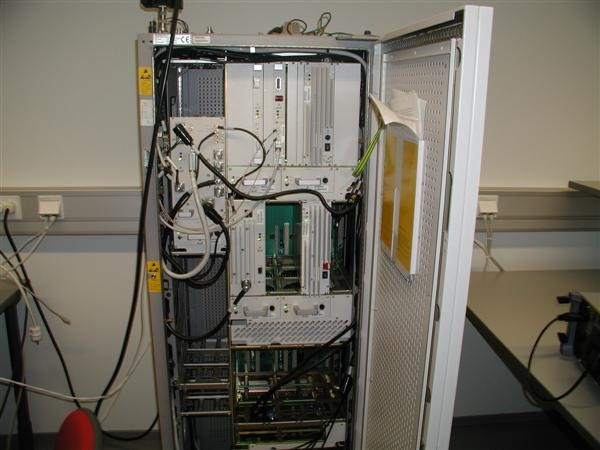
\includegraphics[scale=0.8]{GSM/Pic1}}
\caption{ Nokia DE/DF 34 Talk-family base station}
\end{figure}
\subsection{MMI Software Structure}
We were using MMI to control the BTS. MMI software is needed to download SW and HW, DB or HW Info files, reset the BTS objects, control BTS tests and devices, and also manage alarms. With the Talk-family BTS MMI, there can be three different windows in the MMI mainframe. It is advisable to always have the Messages and Alarms window open. This makes working with the MMI more efficient.
\subsection{Digital Radio Communications Tester CMD57}
Digital Radio Communications tester CMD 57 is an advance top class instrument for measurements on base stations (BTS) and base station modules. (fig. 2)
\begin{figure}
\centerline{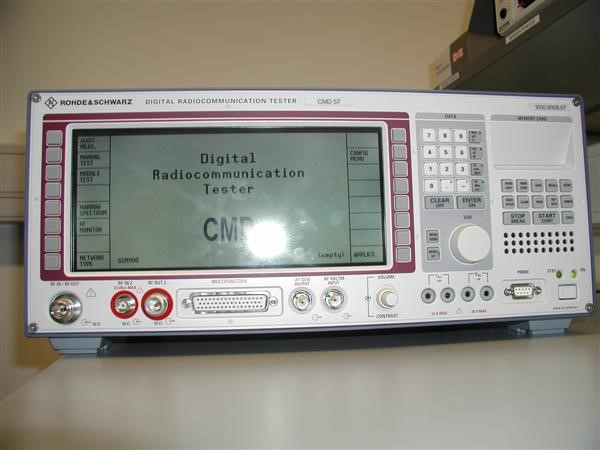
\includegraphics[scale=0.8]{GSM/Pic2}}
\caption{Rohde \& Schwarz Digital Radio Communications Tester CMD 57}
\end{figure}
CMD 57 is designed for measurements in line with:
\begin{itemize}
\item GSM900
\item E-GSM
\item UIC-European train radiotelephony
\item GSM1800
\item GSM1900 optionally
\end{itemize}
The main applications are:
\begin{itemize}
\item Module testing in production
\item Final testing with Abis control
\item Installation with Abis control
\item Service with test mobile functionality
\end{itemize}
CMD 57 allows measurements on transmitters and receivers of base station without affecting telephone calls in progress.
\section{Calibrating Of the Cables Attenuators}
Measurement equipment: CMD57 and spectrum analyser\\\\
The settings of the spectrum analyser:
\begin{itemize}
\item Set the frequency
\item Span 0 Hz
\item Sweep 10ms
\item VBW 300kHz
\item RBW 300kHz
\item Trace average
\end{itemize}
Settings of the CMD57:
\begin{itemize}
\item Module test
\item RF Gen
\begin{itemize}
\item Frequency
\item Offset 0 Hz
\item RF-level –50dBm
\end{itemize}
\item Connect/ext att
\begin{itemize}
\item Select ports and attenuation
\end{itemize}
\item Select correct GSM network type
\end{itemize}
CMD sends when MENU is pressed.
\section{Powering Up the Base Station}
We turned the power on both PSUA-units on the base station.
\section{Base Station and MMI Software}
We connected the 13MHz Test signal of the BTS to the REF-port of the CMD57 and CMD57 RF In/Out to the ANT. 1 connector of the base station. Also connected a serial cable from PC’s serial port to the BTS’s MMI-test-port. When the power is on there is a text 0005 at the display of BCF and POFF/HOP at the display of TRX.\\\\
Then, we started the MMI-program: Start/Programs/BTS MMI Software/BTS MMI and disabled Abis-interface: Object/Disable A-bis.\\\\
When device status is BCF00 SW Loading (fig. 3), we selected BTS SW/Use Current SW Packet. BTS is ready for testing, when device status is BCF00 Supervisory. (fig. 4)
\begin{figure}
\centerline{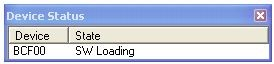
\includegraphics[scale=1]{GSM/Pic3}}
\caption{SW Loading}
\end{figure}
\begin{figure}
\centerline{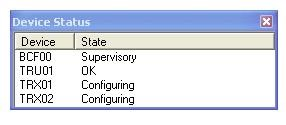
\includegraphics[scale=1]{GSM/Pic4}}
\caption{BCF00 Supervisory}
\end{figure}
\section{TRX Loop Test}
\begin{figure}
\centerline{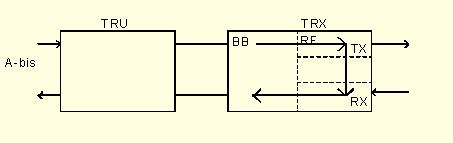
\includegraphics[scale=1]{GSM/Pic5}}
\caption{TRX loop scheme}
\end{figure}
MMI: From the MMI program we chose: Test / Send BCCH Carrier (fig. 6)
\begin{figure}
\centerline{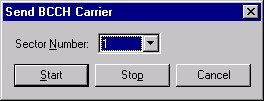
\includegraphics[scale=1]{GSM/Pic6}}
\caption{Options for BCCH Carrier}
\end{figure}
\begin{figure}
\centerline{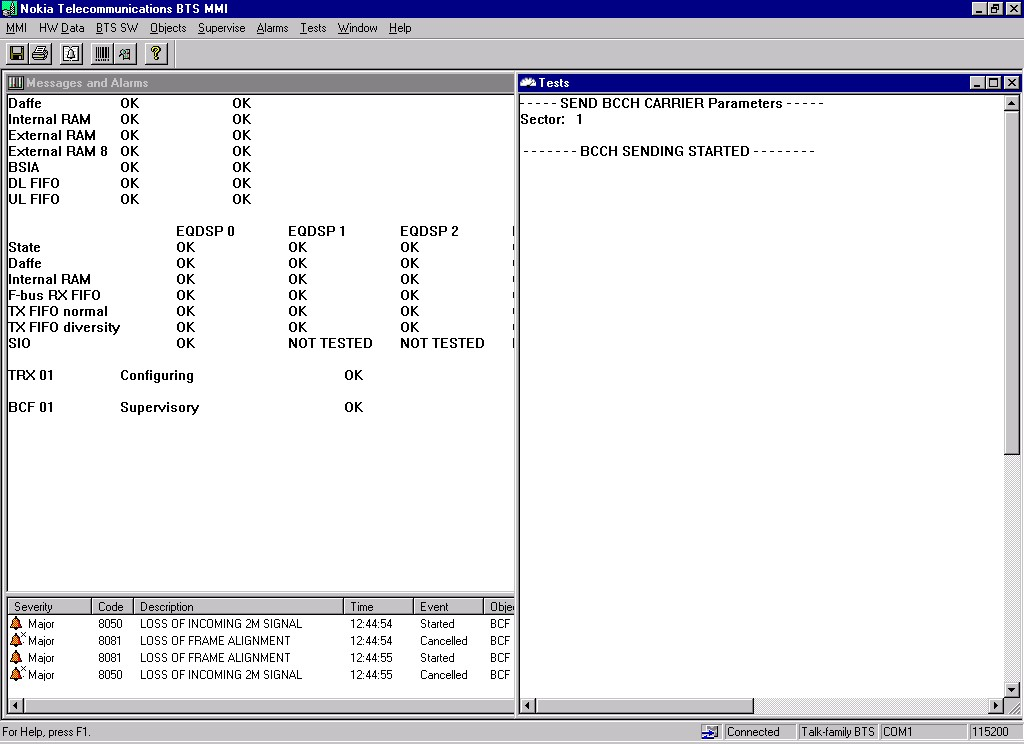
\includegraphics[scale=0.5]{GSM/Pic7}}
\caption{BCCH sending started}
\end{figure}
\subsection{MMI: Test/ TRX Loop Test}
\begin{figure}
\centerline{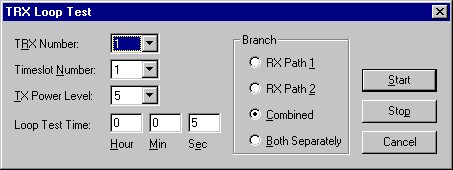
\includegraphics[scale=1]{GSM/Pic8}}
\caption{TRX Loop Test Example}
\end{figure}
After choosing values we pressed Start and then we tested both of the TRX’s and used different timeslots and TX Power Levels and at the end of the TR LOOP test we chose Test / Send BCCH Carrier and clicked Stop.
\begin{figure}
\centerline{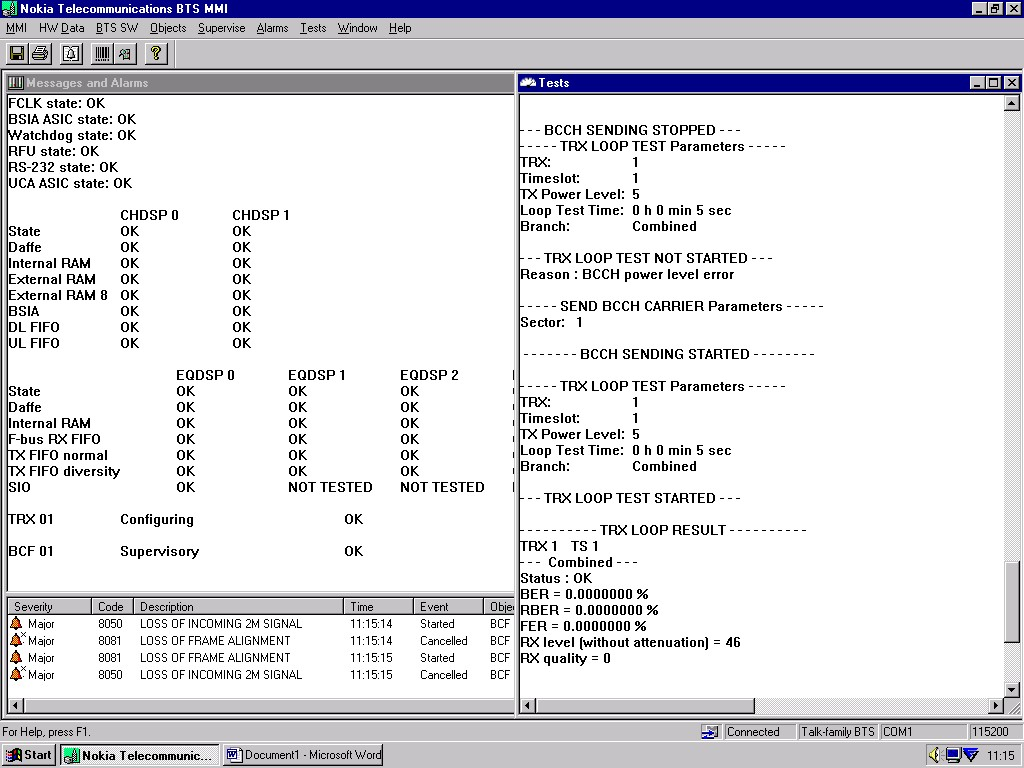
\includegraphics[scale=0.4]{GSM/Pic9}}
\caption{TRX Loop test result}
\end{figure}
\section{Test Pattern Transmission}
\paragraph{MMI:}
\begin{itemize}
\item Tests / Send BCCH Carrier
\item Test / Test Pattern Transmission
\end{itemize}
We chose the ARFN number 521 (GSM1800) and set only the one timeslot using different TX Power levels, bit patterns and timeslots. (Fig. 10)
\begin{figure}
\centerline{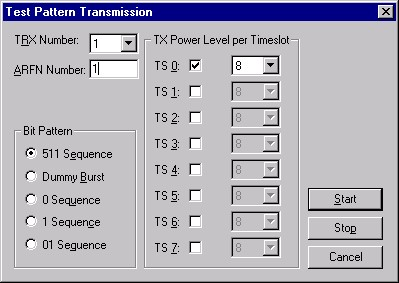
\includegraphics[scale=0.8]{GSM/Pic10}}
\caption{Test Pattern Transmission}
\end{figure}
\paragraph{CMD: Module test}
Also we have done Power Ramp Test, and checked that power ramp is correct. (fig. 11) and
phase frequency test. There, we checked that phase frequency is correct. (fig. 12)
\begin{figure}
\centerline{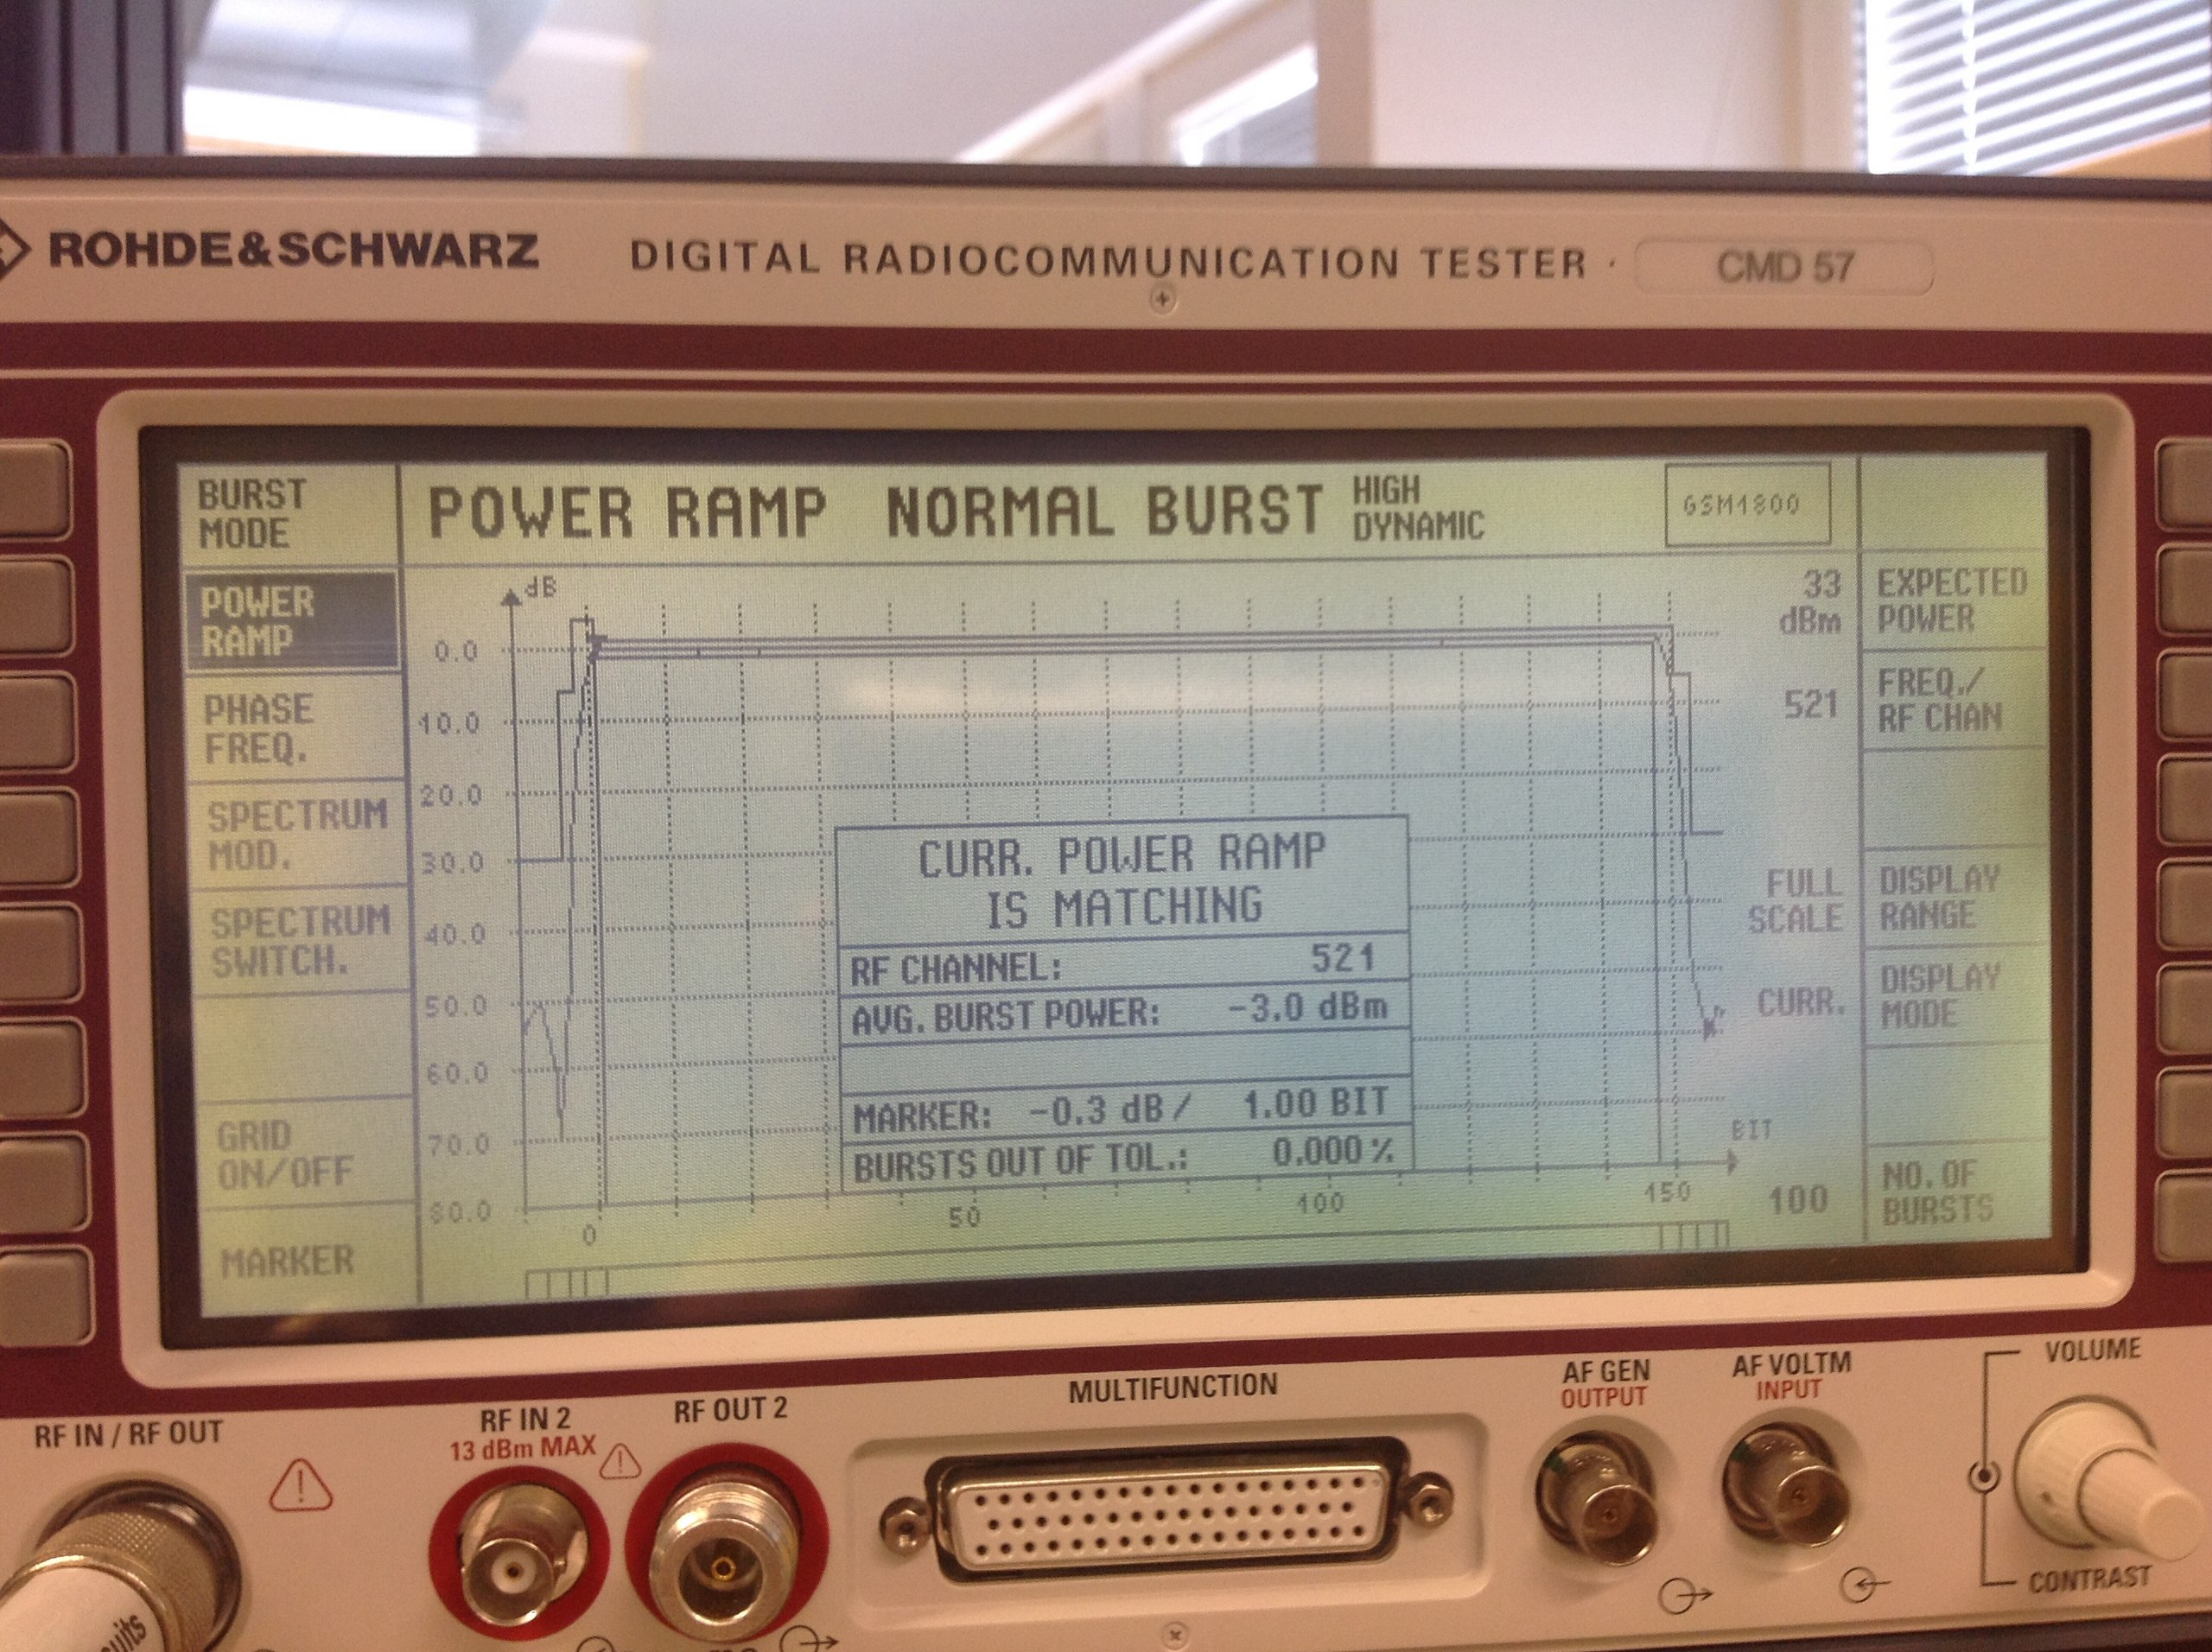
\includegraphics[scale=0.1]{GSM/Pic11}}
\caption{Power Ramp Test result}
\end{figure}
\begin{figure}
\centerline{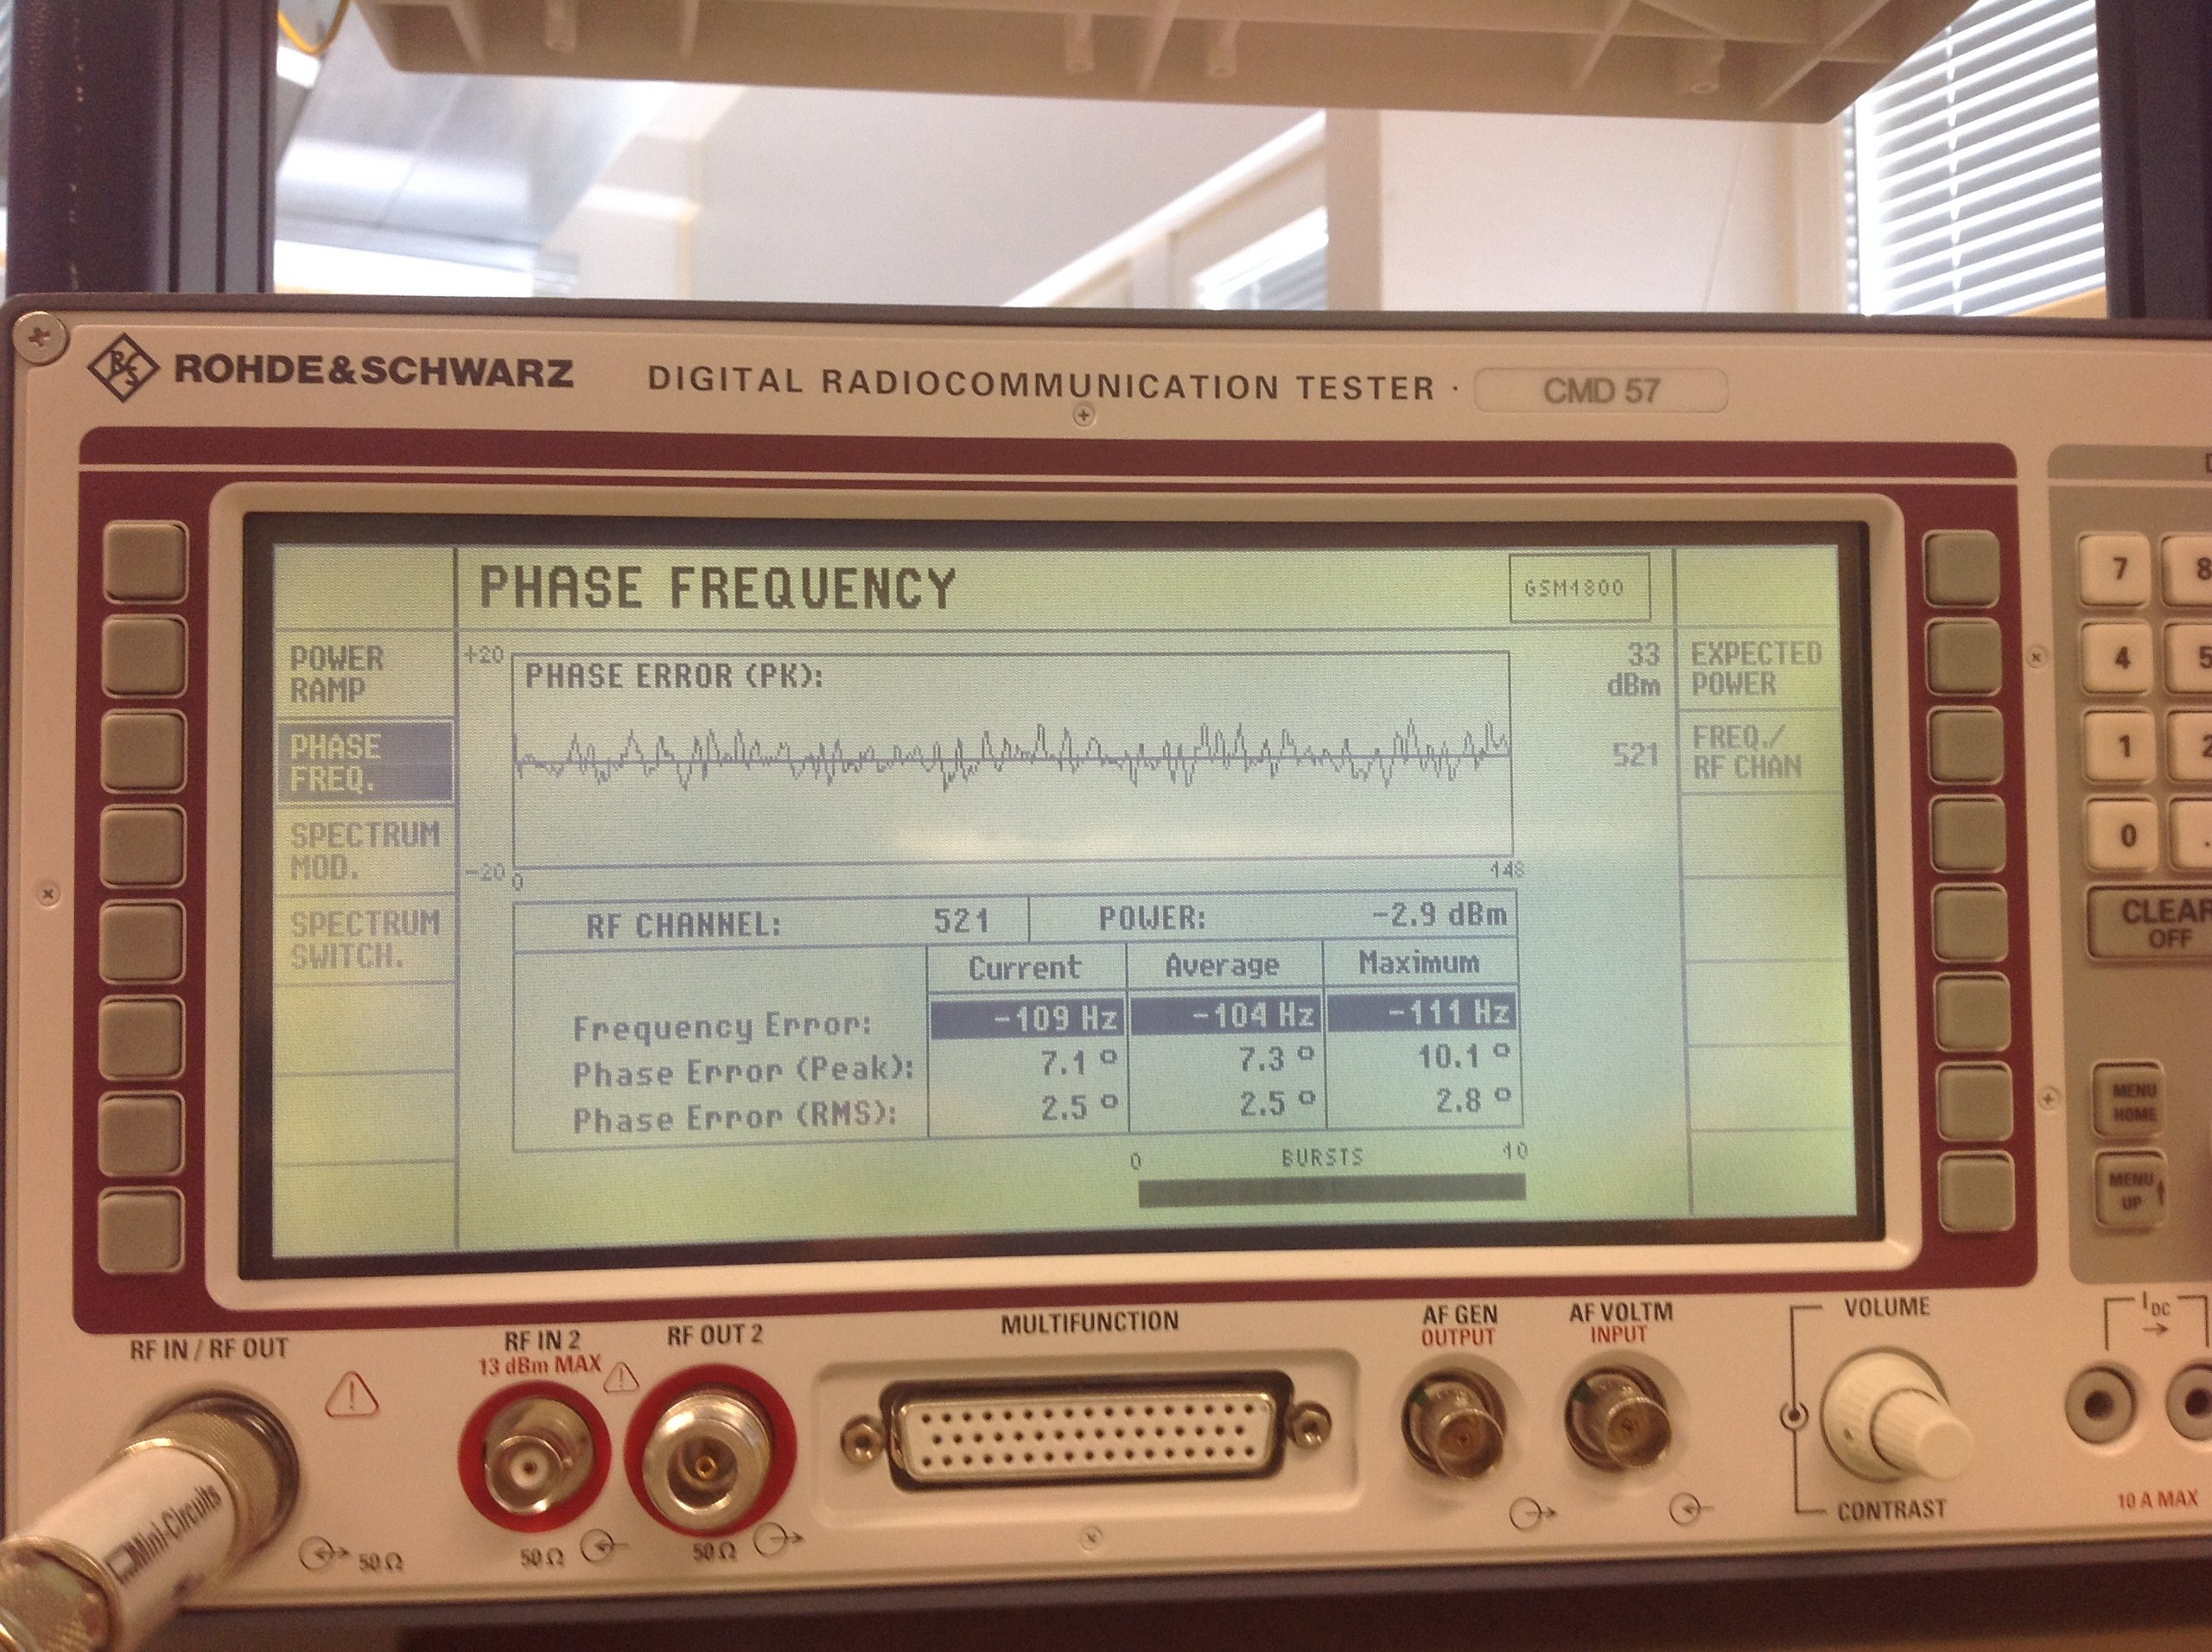
\includegraphics[scale=0.1]{GSM/Pic12}}
\caption{Phase Frequency Test result}
\end{figure}
In the end of measurement we went back to MMI Program and chose Tests/Test Pattern Transmission and clicked Stop and Tests/Send BCCH Carrier and clicked Stop.
\section{Air Interface Loop Tests}
\begin{figure}
\centerline{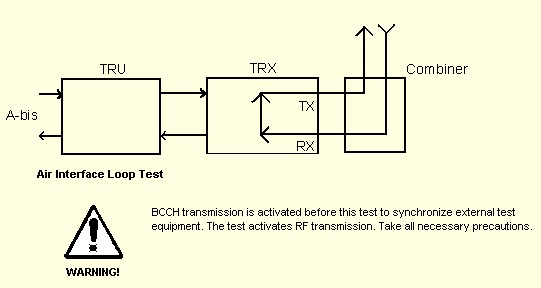
\includegraphics[scale=0.8]{GSM/Pic13}}
\caption{Air Interface Loop scheme}
\end{figure}
\begin{itemize}

\item MMI: Test\/Send BCCH carrier
\item We set the correct timeslot and the channel.
\item CMD57: Manual tests
\item Pressed Try to sync
\end{itemize}
Display has to show search for signals and BTS power level. Unfortunately, we had difficulty synchronizing, so we couldn’t finish this test.
\section{BER (Bit Error Rate) Test}
Also, we couldn’t make BER test due to synchronization.
\end{document}
